%$Id: tutor.tex 3 2014-07-31 09:59:20Z kruegerh $
%;;; Local IspellDict: "british"

\section{Tutorials}

I recommend to work step-by-step through some of the examples, to learn about some special features in GPLIGC.
The used igc-files can be found at the download section of the GPLIGC webpages.

\subsection{GPLIGC -- competition flight analysis  of 482zc251.igc}

\subsubsection{482zc251.igc}
This flight has been done at the third day of the Klippenenck-Competition 2004.
I won this day 0.1~km/h faster than the second pilot in the 15~m FAI class. The plane was a ASW20.
You can download the igc file of this flight from the GPLIGC web site (download/examples), to practice using GPLIGC.

\subsubsection{General information, altitude calibration}
Right after opening the igc file in GPLIGC, we will see a lot of confusing waypoints (fig.~\ref{flightview}).
What has gone wrong can be seen in the flight information window (fig.~\ref{flightinfo}).
The flight information window shows all the header lines which are contained in the igc file.
We can check all available information about pilot, plane and logger here.
We also can see, that two tasks are defined, the one from the previous competition days is still present in the file.
We will open the task editor window (fig.~\ref{taskeditor}) and delete all waypoints from the previous days task.
The remaining task should look like \texttt{AP 3 TUTTLING - KIRNBERGSEE - FREUDENSTADT - HOHENZOLLERN - HARBURG - ZL 2 KLIPPENE}.
The flight view window will show the task like this (fig.~\ref{flightview2}).
The altitude measurement of the logger uses a fixed reference pressure.
To get valid MSL altitudes we have to calibrate the data.
As we know the elevation of Klippeneck airfield (970m MSL) we can do this easily.
We have to find a logged position (by left-clicking in the flight view windows barogram strip or using F1-F4 to move the cursor),
where the plane was on the airfield, right before take-off. Logged altitude is about 920m.
Then we have to press \texttt{e} and enter the real altitude of this position (970m).
Now the calibration has been done.

\subsubsection{Starting and finishing time, overall task speed, task distance}
To determine the overall task speed we have to define the time of crossing the starting line as well as the time of reaching the finishing line.
To do this we will zoom (drag a zooming box using the right mouse button) into the starting point/line (fig.~\ref{start}).
We have to find the last position before the plane crossed the starting line.
We will find this at 11:02:03 UTC. To define this as starting point we press \texttt{s} with the cursor marking this position.
The starting position will be marked with a black circle after this procedure.
The altitude of the plane while crossing the starting line was 1930m which is below the limit of 2000m, but the groundspeed of 165km/h exceeds the 150km/h limit,
but luckily I did not get any penalty points for that.

Now, we zoom out (pressing \texttt{z}) and then in again (dragging a box with right mouse button) to magnify the area at the finish.
We will find the first point after crossing the finishing line at 15:47:16 (fig.~\ref{finish}) and mark it with \texttt{f}.
A black circle is shown here also.

After defining the start and finish times we can open the flight statistics window (fig.~\ref{flightstatistic}).
The first part shows information on the flight (take-off and landing time,
total time of flight) and also the defined task start and finishing times and total time of task.
The second part of the window gives information of the task, as defined in the task editor.
The overall task speed is calculated from the task distance and the total time of task.
In this case it was a 434.93km task, done with 91.5km/h. The third part of this information window gives a rough determination of the flown task.
A waypoint is considered as reached if there is any position closer than 3km.
The first point, which is closer than 3km is used for this statistics.
For each leg of the task some information are given. For exact analysis of speeds for some legs you should use the F5,F6,F7 statistics (see \ref{f5f6f7}).

\subsubsection{Thermal and glide statistics}
Pressing \texttt{F8} or \texttt{F9} in the flight view window will open a list of thermals (fig.~\ref{thermals}) or a list of glide distances (fig.~\ref{glide}).
Additional to each list another small statistics window is opened. The lists and statistics will be evaluated between the set start and finish time.
The thermal statistic points out, that we gained 8272m of altitude while circling in 25 thermals. The best one had a lift of 3.44m/s, the worst 0.67m/s.
The average lift was 1.64m/s (this is calculated from total altitude climbed and total time spend circling).
The time spend circling is given in percent of the overall task time. The best lift was only used to climb 220m, as can be seen in the list of thermals.
Double clicking of items in the list will set the cursor to the associated thermal.
This way we can find out, that the most altitude (616m) was gained at a lift of 1.7m/s at the last waypoint (\texttt{HARBURG}).
In this uplift I was circling 11 times to the right which needs 6 minutes.

The list with gliding distances shows, that the longest gliding distance was the final glide of 33km.
It took me 12 minutes with an average descending speed of 1.95m/s. The average speed was 165km/h, the average heading was 245$^\circ$.
Average L/D ratio is calculated to 24. Another very nice glide can be found at 12:01:59.
It only needs 5.5 minutes at 159km/h to fly 14.6km with an average L/D ratio of 88.
The small glide statistics window provides some sums of the gliding list.


\subsubsection{F5,F6,F7 statistics and measuring tool}
\label{f5f6f7}
To get some statistics between some positions the \texttt{F5,F6,F7} tool can be used.
We'll now get some exact information for the second leg (from \texttt{KIRNBERGSEE} to \texttt{FREUDENSTADT}.
We'll find the last point in the FAI sector of \texttt{KIRNBERGSEE} at 11:24:27. This can be marked as first point \texttt{F5}.
A green circle will show up. The second point (reaching FAI sector of \texttt{FREUDENSTADT} 11:59:05) will be defined using \texttt{F6}.
Another green circle will mark this position, and the range between the first and the second point is shown in red (barogram).
Now we can get some statistics between these points by pressing \texttt{F7}.
The result show that the average speed was 103km/h, although I gained 293m.


\subsubsection{OLC flight optimisation}
We would like to evaluate the olc scoring distance of the flight. Therefore we have to set the start
point (pressing \texttt{s}) to the release from tow, and the finish time (pressing \texttt{f}) to the landing time.
I found 10:15:07 for release and 15:47:43 for landing. Now we can start the optimisation from the task editor.
The optimisation will find the best olc-task between the release and the landing time. It's 438.14km.

% not valid anymore
%After selecting olc flight claim from task editor window, we have to fill in some details. Also we can chose to use the GPLIGC optimised task, or to let the optimisation up to the olc-server. Subsequently GPLIGC will point us to the olc-website, where we could finish the flight claim.


% old!
% \begin{figure}[h]
% \caption{\label{main}The GPLIGC main window}
% \begin{center}
% 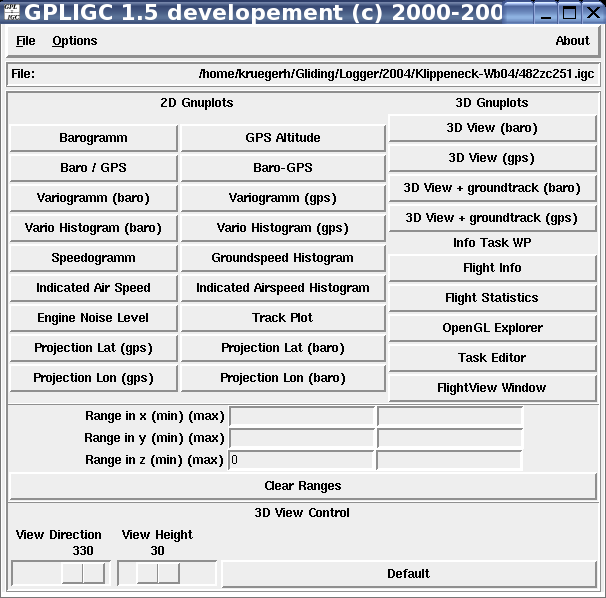
\includegraphics[width=\textwidth]{png/gpligc-main}
% \end{center}
% \end{figure}



\begin{figure}[h]
\caption{\label{flightview}The GPLIGC flight view window showing a flight with two tasks}
\begin{center}
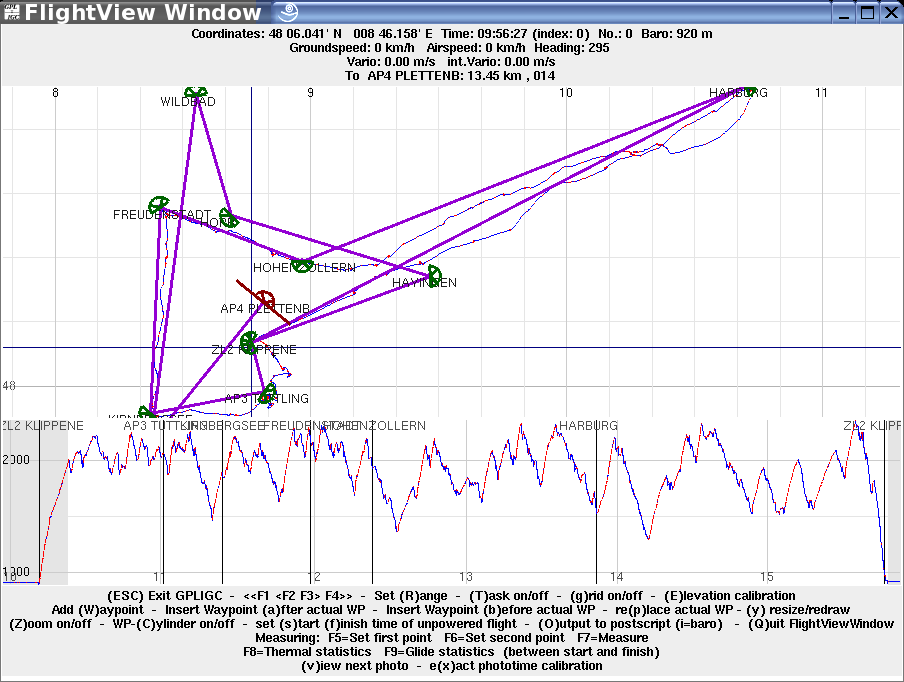
\includegraphics[width=\textwidth]{png/flightview-1}
\end{center}
\end{figure}

\begin{figure}[h]
\caption{\label{flightinfo}The GPLIGC flight info window}
\begin{center}
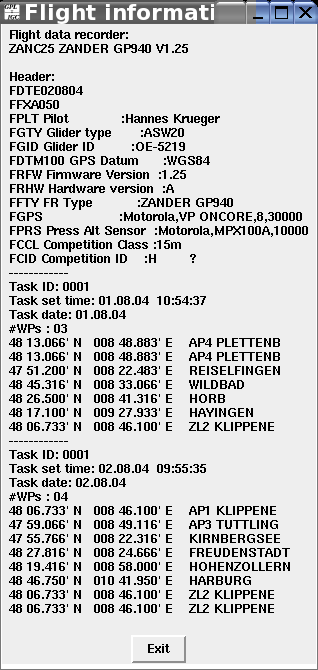
\includegraphics{png/flightinfo}
\end{center}
\end{figure}


\begin{figure}[h]
\caption{\label{taskeditor}The GPLIGC task editor window}
\begin{center}
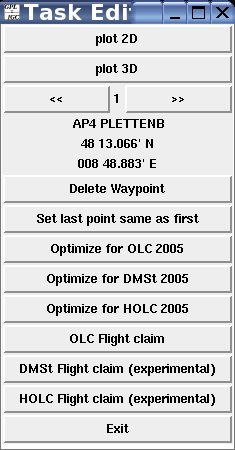
\includegraphics{png/taskeditor}
\end{center}
\end{figure}

\begin{figure}[h]
\caption{\label{flightview2}The GPLIGC flight view window, with the valid task}
\begin{center}
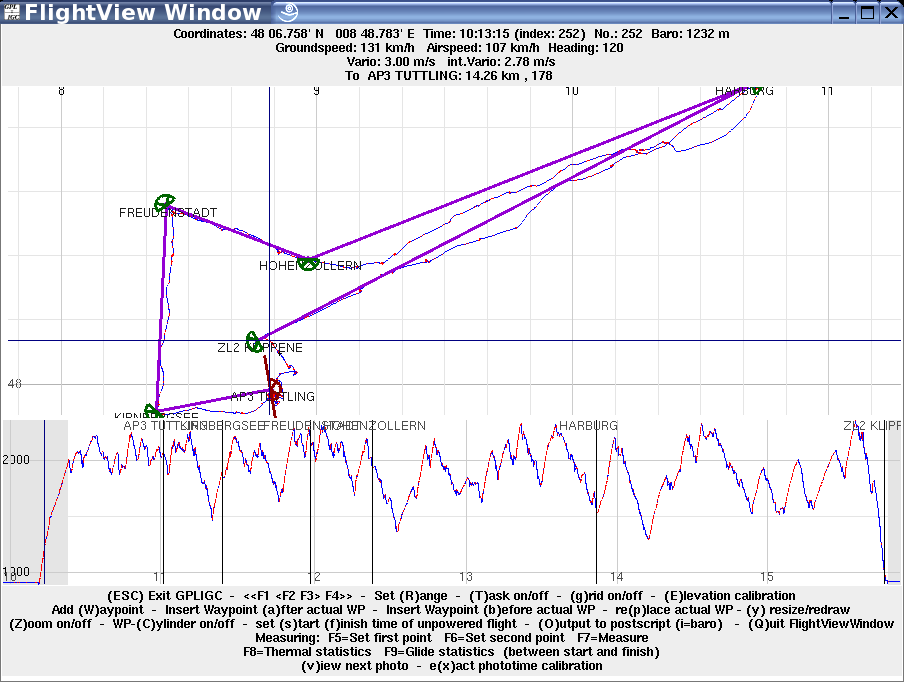
\includegraphics[width=\textwidth]{png/flightview-2}
\end{center}
\end{figure}

\begin{figure}[h]
\caption{\label{start}Crossing the starting line}
\begin{center}
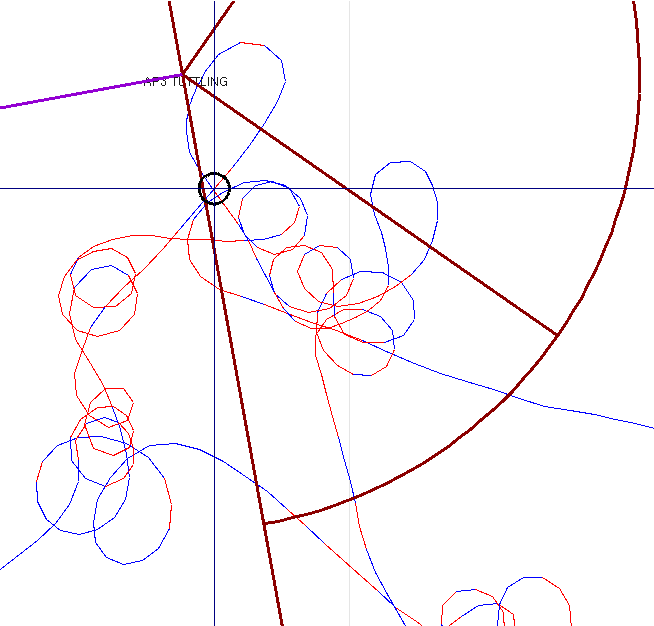
\includegraphics[width=\textwidth]{png/start}
\end{center}
\end{figure}

\begin{figure}[h]
\caption{\label{finish}Reaching the finishing line}
\begin{center}
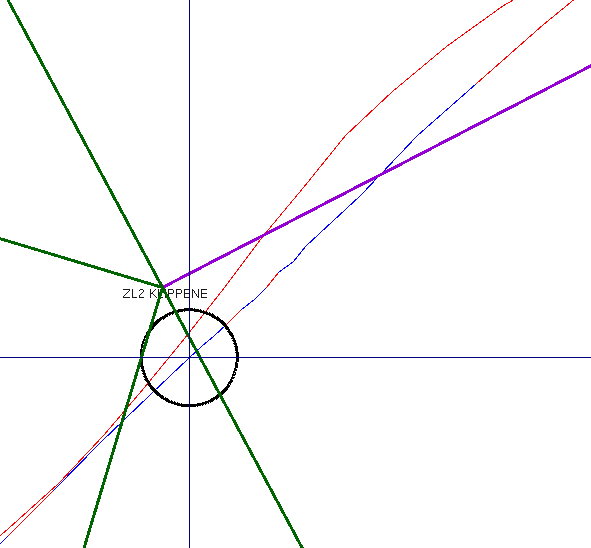
\includegraphics[width=\textwidth]{png/finish}
\end{center}
\end{figure}

\begin{figure}[h]
\caption{\label{flightstatistic}The GPLIGC flight statistic window}
\begin{center}
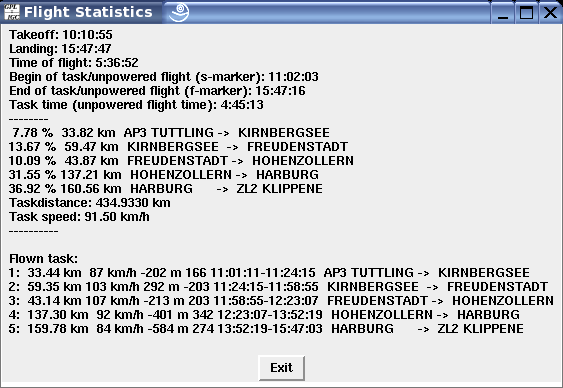
\includegraphics[width=\textwidth]{png/flightstatistic}
\end{center}
\end{figure}

\begin{figure}[h]
\caption{\label{thermals}The GPLIGC thermal statistics}
\begin{center}
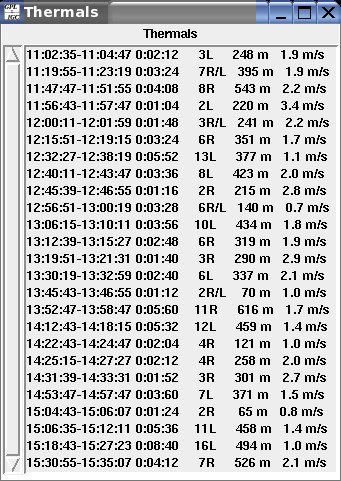
\includegraphics[height=13cm]{png/thermstat}
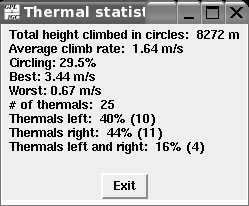
\includegraphics{png/thermstat2}
\end{center}
\end{figure}

\begin{figure}[h]
\caption{\label{glide}The GPLIGC glide statistics}
\begin{center}
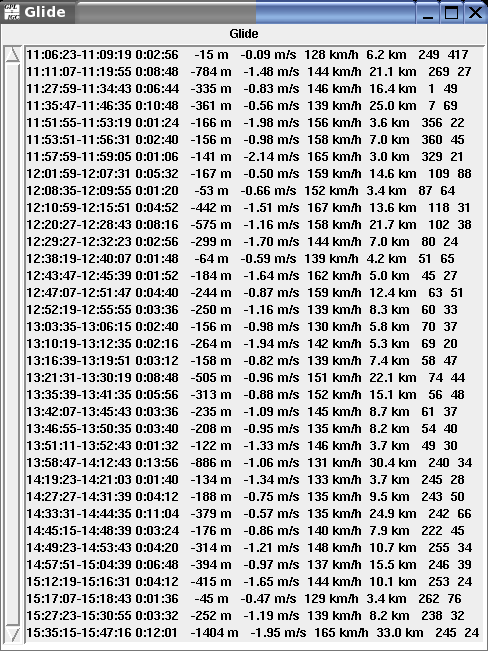
\includegraphics[height=13cm]{png/glidestat1}
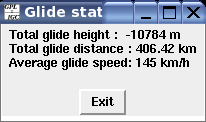
\includegraphics{png/glidestat2}
\end{center}
\end{figure}


\clearpage


\subsection{Innsbruck F\"ohn flight 2009-04-16-GAR-000-02.igc}

This nice example of a classical Innsbruck F\"ohn flight was done with our club DuoDiscus T in april 2009.

\subsubsection{Flight Information (additional)}
This tool allows us to enter/update some additional information. The date is shown correct, but the pilots name is missing.
Plane and callsign can be entered too, the QHN can be set to 1006 (if I remember right). The timezone is +2, and the airfield is Innsbruck (LOWI).

\subsubsection{Calibration of the altitude}
The track was recorded with a Garmin Geko 301.
Using the Flight View Window (fvw) the cursor can be set some point right before the take-off (e.g. 13:35).
As can be seen here, the recorded altitude is quite close to 580m (which is the elevation of Innsbruck airport). The Geko's
auto calibration function did a good job (it corrects the reference pressure with averaged GPS altitudes).
Subsequently, the right elevation of Innsbruck LOWI (580~m) can be entered by pressing \texttt{e}. If the \emph{save} button of the additional flight information tool is used, the calibration is saved and will be available later (after opening this file again). In this case the calibration is not really needed, since the offset is ca. three or four meters, only.

\subsubsection{Winch}
Using the fvw and the cursor (move with F1-F4 or with the mouse), the winch take-off can be found between 13:35:26 and 13:36:05. To analyse the winch launch mark the first point with F5, the second with F6. Statistics is then calculated with F7.
The launch took 42 seconds, the gain in altitude was 343~m with an average climbing rate of 8.2~m/s. The heading was 81$^\circ$, which is in good agreement with the runway 08. The speed of 91 km/h looks too small for a DuoDiscus, but the value reflects the projected groundspeed, not the airspeed. Change in altitude and the wind is not taken into account.

\subsubsection{Ridge soaring}
The lift at the ridge was entered at 13:36:38 and until 13:43:35 (within 7~min) 1700~m were gained in an average lift of 4.1~m/s with a nice maximum of ca. 8~m/s.

\subsubsection{Wave}
The first climb in the wave was found (after ATC clearence) at 13:56:20. In the following 10~min, ca.~1700m with an average of 2.8~m/s were climbed to the maximum of the ATC clearence. Subsequently airbrakes had to be used to limit the altitude.
As you can see in the barogram I really enjoyed beeing on top (for more than one hour). A feet heating device helped to stay warm at about -20$^\circ$C, and of course oxygen was used. Figure~\ref{foehngap} shows the view to the wave clouds and the typical foehn gap above the Inn valley.
The pictures are not included in the example, but the photo-locator option would look like Fig.~\ref{pic88}, showing the positions of the pictures. Btw. Fig.~\ref{pic88} was created using the postscript output from fvw via the keys \texttt{o} and \texttt{i}.

\begin{figure}[h]
\caption{\label{foehngap}Foehn gap and massive wave clouds above the Inn valley. The picture was taken in ca.~5000~m, the top of the Ac Len is probably higher than FL200.}
\begin{center}
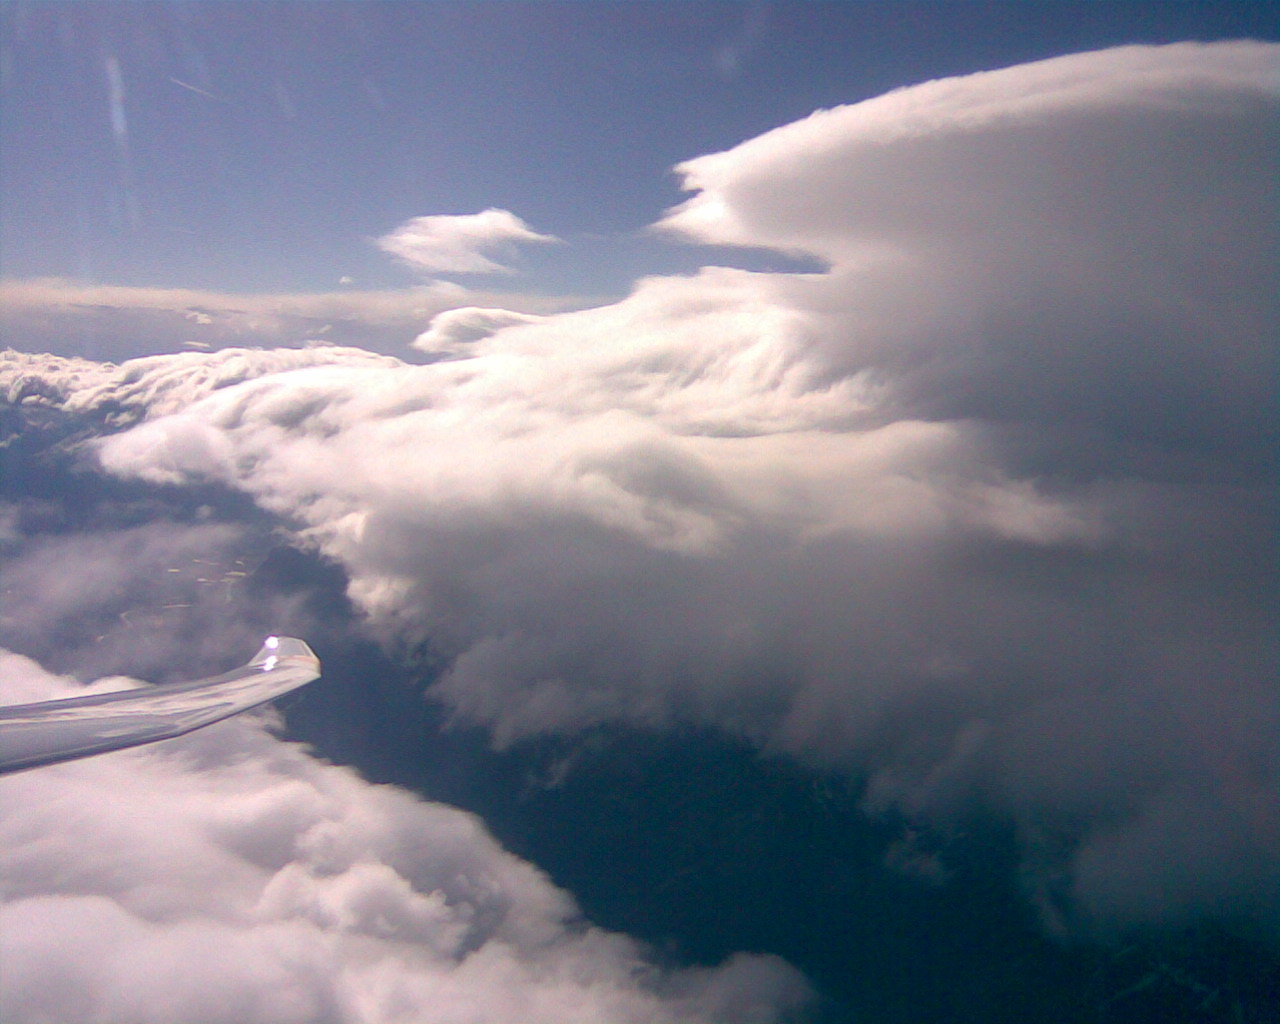
\includegraphics[width=\textwidth]{png/Bild088.jpg}
%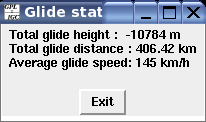
\includegraphics{png/glidestat2}
\end{center}
\end{figure}

\begin{figure}[h]
\caption{\label{pic88}Locating pictures}
\begin{center}
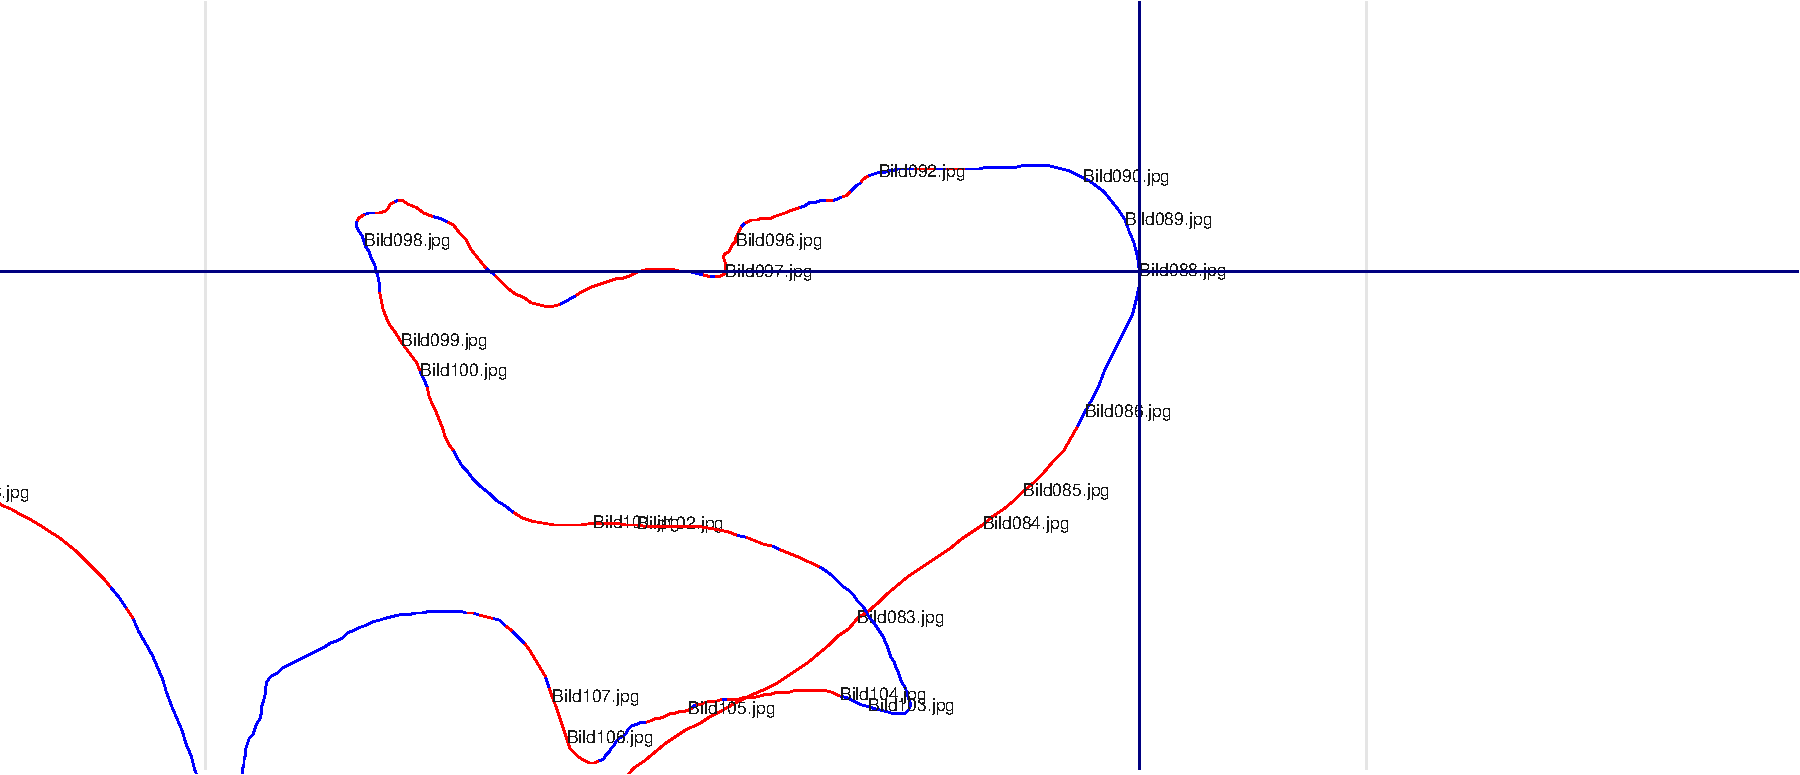
\includegraphics[width=\textwidth]{png/pic88fvw}
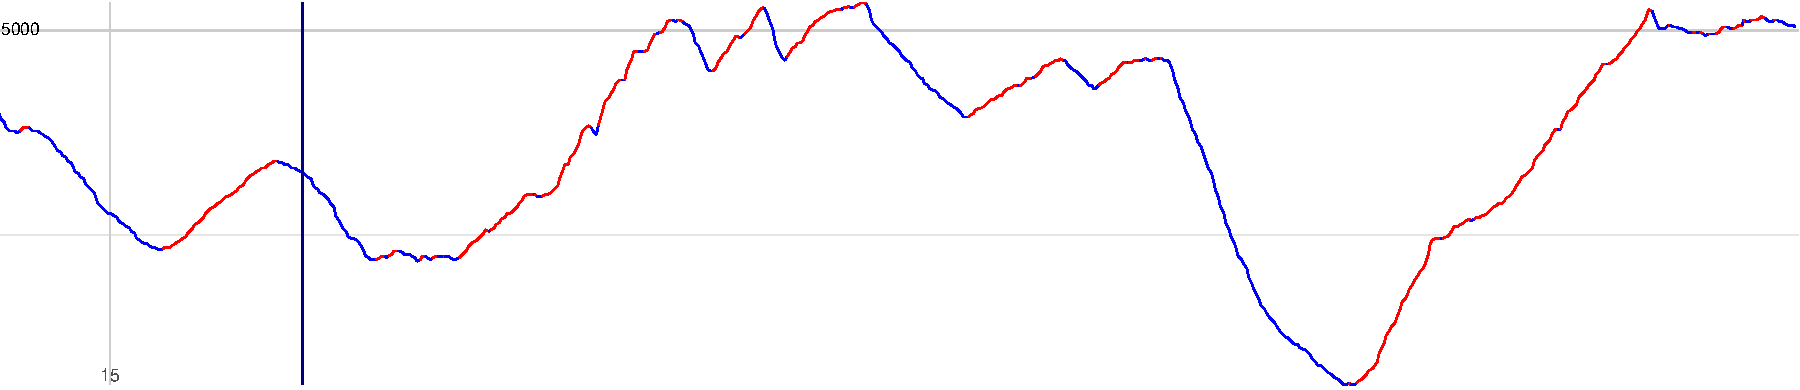
\includegraphics[width=\textwidth]{png/pic88fvwbaro}
\end{center}
\end{figure}


\subsubsection{Analysis of wind}
To analyse the wind, which causes such nice lifts, we have to select parts of the track including many different directions flown. Circling works very well, but some figure-of-eight turns can be used too.
13:36:29--13:39:35 corresponds to the first lift at the ridge up to ca.~1500m. Selecting this range (F5/F6) and pressing F7 will analyse the wind. The opened gnuplot window, shows how the groundspeed depends on the heading (if airspeed is recorded -- as e.g. in some Zander loggers -- the difference groundspeed-airspeed is used). A sinus function is fitted to the data, which gives the direction and speed of the wind. In this case its ca.~40km/h from 137$^\circ$. The direction is typical for this part of the Inn valley in foehn situations.

Another interesting part is from 14:06:29 to 14:18:53, which includes some circles and figure-of-eight turns in the wave just north of Nockspitze and Axamer Lizum. The analysis shows a wind from 190$^\circ$ with 50km/h only, which is surprisingly low for such a strong wave.
The wave north of the Glungezer (14:25:14--14:56:32) shows a bit higher wind speed of 60km/h and ca.~200$^\circ$.
The second ascend to the wave level (16:38:23--16:57:08) exhibits very similar wind conditions.

\subsubsection{Oxygen debriefing}
The \emph{Flight Statistics} window shows some information on (recommended) oxygen consumption. It is calculated for constant open-flow systems. The values in brackets corresponds to the use of an Oxymizer canula (ca.~1/3 of a regular open-flow system).
According to the FAR regulation 91.211 a total of 226~l of oxygen should have been used. Starting to use oxygen at FL100 (as recommended) would have increased the total to 275~l. Using an Oxymizer canula would have reduced these amounts to ca.~1/3.
However, modern pulse-demand systems save even more oxygen, depending on your breathing rate.


\clearpage

\subsection{using loopviewer.pl to make presentations of flights}

loopviewer.pl is a simple script, which uses ogie to show flights automatically.
This could be used for presentation of flights, e.g. at competitions.
loopviewer.pl reads a list, which contains two entries (enclosed in ") per line:
the first is the path and name of the igc-file, the second a comment, which should be shown with the flight.
So far, this simple script needs manual editing, to obtain a reasonable set of parameters.


%\begin{enumerate}
%\item Step 1
%\item Step 2
%\item ...
%\end{enumerate}


%%% Local Variables:
%%% mode: latex
%%% TeX-master: "GPLIGC_manual"
%%% End:


%;;; Local IspellDict: "british"
%%% Local Variables:
%%% mode: latex
%%% TeX-master: "GPLIGC_manual.tex"
%%% End:
